\documentclass[a4paper,11pt]{article}
\usepackage[utf8]{inputenc}
\usepackage{lastpage}
\usepackage{fancyhdr}
\usepackage[english]{babel}
\usepackage[a4paper,margin=1in]{geometry}
\usepackage{multirow}
\usepackage[table,xcdraw]{xcolor}
\usepackage{array}
\usepackage{amsmath}
\usepackage{graphicx}
\usepackage{caption}


\graphicspath{ {images/} }

\newcolumntype{L}[1]{>{\raggedright\let\newline\\\arraybackslash\hspace{0pt}}m{#1}}
\newcolumntype{C}[1]{>{\centering\let\newline\\\arraybackslash\hspace{0pt}}m{#1}}
\newcolumntype{R}[1]{>{\raggedleft\let\newline\\\arraybackslash\hspace{0pt}}m{#1}}

\newcommand\tab[1][4mm]{\hspace*{#1}}


%-------------------------------------------------------------------------------
% HEADER & FOOTER
%-------------------------------------------------------------------------------

\pagestyle{fancy}
\fancyhf{}
\setlength\headheight{15pt}
\fancyhead[L]{ HPC Assignment 2 }
\fancyhead[R]{Student ID: 100633486}
\fancyfoot[R]{Page \thepage\ of \pageref{LastPage}}


%-------------------------------------------------------------------------------
% TITLE PAGE
%-------------------------------------------------------------------------------

\begin{document}

\title{
	\Huge \textbf {Langevin Dynamics, Part I}
    \\ [0.2cm]
	\LARGE HPC Assignment 2 - Feb, 2017
    \\ [0.5cm]
    \hrule
}

\date{}

\author{
		\Large Kamyar Nazeri \\
		\large Student ID: 100633486 }

\maketitle
\newpage

\section*{Introduction}
In this assignment, we are simulating the Langevin dynamics in its simplest form and perform tests on the code and analyze the output data to build confidence in correctness and accuracy of our simulation. \\
The following restrictions are imposed in our simulation:
\begin{itemize}
  \item Particle trajectories are implemented in 2D.
  \item No interaction exists between the particles.
  \item Equation is equipped with periodic boundary conditions.
\end{itemize}
\textit{Note: There’s no implicit vectorized code in C++, hence the particles initialization is done by creating a data-structure and explicit loop over elements. Today's modern C++ compilers (including gcc and Intel's compilers) automatically generate vectorized code as part of their optimizations\cite{vectorization}} \\\\
\section*{The Langevin Equation:}
The Langevin equation describes Brownian motion, the random movement of a particle in a fluid due to collisions with the molecules of the fluid:
\begin{equation*}
  m\ dv = -\gamma v\ dt + \sqrt{dt}\ c\ \eta(x,t)
\end{equation*}


Where \(v \in R^2\) is a velocity of a particle and is implemented in our code using \emph{Velocity Verlet algorithm}\cite{verlet} and \(\eta\) is the noise term which we implement using \emph{Intel MKL}\cite{mkl} library to generate random numbers with normal (Gaussian) distribution. As a consequence of the fluctuation-dissipation theorem for this system, we have \(c = \sqrt{2\gamma k_BT} \) where \(k_B\) is \emph{Boltzmann}'s constant and \(T\) is the temperature. \\\\
In the code \(m\), \(\gamma\) and \(k_BT\) are set to unity, we start nondimensionalizing the above equation to show how setting system parameters to unity makes sense: \\
\begin{equation*}
m\ \frac{dv}{dt} = -\gamma v\ + \frac{c}{\sqrt{dt}}\ \eta(x,t)
\end{equation*}
Parameters: \(m\), \(\gamma\), \(c\) \\
Variables: \(x\), \(t\)\\
We are finding dimensionless parameters \(\hat{x}\) and \(\hat{t}\) in terms of \(m\), \(\gamma\) and \(c\) (\emph{note that \(\eta\) is a dimensionless random scalar value}) \\

set: \(\hat{x} = \frac{x}{x_s}\) \tab,\tab \(\hat{t} = \frac{t}{t_s}\) \tab,\tab \(\hat{v} = \frac{v}{v_s}\) \tab (\small \(x_s\), \(t_s\) \emph{and} \(v_s\) \emph{have dimensions}) \\
\begin{align*}
   &m\ \frac{d^2x}{dt^2} = -\gamma \frac{dx}{dt}\ + \frac{c}{\sqrt{dt}}\ \eta(x,t) \Rightarrow m\ \frac{d^2(\hat{x}\ x_s)}{d(\hat{t}\ t_s)^2} = -\gamma \frac{d(\hat{x}\ x_s)}{d(\hat{t}\ t_s)}\ + \frac{c}{\sqrt{d(\hat{t}\ t_s)}}\ \eta(x,t)
   \\
   &\frac{m\ x_s}{t_s^2} \frac{d^2\hat{x}}{d\hat{t}^2} + \frac{\gamma\ x_s}{t_s} \frac{d\hat{x}}{d\hat{t}}\ - \frac{c}{\sqrt{t_s}\sqrt{d\hat{t}}}\ \eta(x,t) = 0
   \\
   &\frac{d^2\hat{x}}{d\hat{t}^2} + \frac{\gamma\ t_s}{m} \frac{d\hat{x}}{d\hat{t}}\ - \frac{c\ t^{3/2}}{m\ x_s}\ \eta(x,t) = 0
   \\
\end{align*}
The goal is to determine \(x_s\) and \(t_s\) so that equations become as simple as possible: \\

    {\framebox{\emph{unit of mass} \(\equiv m \)}} \\

    \(\frac{\gamma\ t_s}{m} = 1 \tab \Rightarrow \tab t_s = \frac{m}{\gamma}\) \hspace{20mm}
    {\framebox{\emph{unit of time} \(\equiv \frac{m}{\gamma} \)}} \\

    \(\frac{c\ t^{3/2}}{m\ x_s} = 1 \tab \Rightarrow \tab x_s=\frac{c\ \sqrt{m}}{\gamma^{3/2}}\) \hspace{12mm}
    {\framebox{\emph{unit of length} \(\equiv \frac{c\ \sqrt{m}}{\gamma^{3/2}} \)}} \\\\
The nondimensionalized form of the original Langevin equation becomes:
\begin{align*}
    &m\ dv = -\gamma v\ dt + \sqrt{dt}\ c\ \eta(x,t) \\
    &m\ d(v_s\ \hat{v}) + \gamma (v_s\ \hat{v})\ d(\frac{m}{\gamma}\hat{t}) - \sqrt{d(\frac{m}{\gamma}\hat{t})}\ c\ \eta(x,t) = 0 \tab \Rightarrow \tab d\hat{v} + \hat{v}\ d\hat{t} + \frac{c}{\sqrt{m\gamma}v_s} \sqrt{d\hat{t}}\ \eta(x,t) = 0
\end{align*}
To simplify the differential equation: \\
    \(\frac{c}{\sqrt{m\gamma}v_s} = 1 \tab \Rightarrow \tab v_s = \frac{c}{\sqrt{m\gamma}}\) \hspace{15mm}
    {\framebox{\emph{unit of velocity} \(\equiv \frac{c}{\sqrt{m\gamma}} = \frac{\sqrt{2\ K_BT}}{\sqrt{m}} \)}} \\\\
\\The final dimensionless differential equation:
\begin{align*}
    d\hat{v} + \hat{v}\ d\hat{t} + \sqrt{d\hat{t}}\ \eta(x,t) = 0
\end{align*}
To simplify our simulation, we declare \(m\), \(\gamma\) and \(k_BT\) to unity, which means we can totally eliminate the units of \(m\) or \(k_BT\) (order of \(10^{-23}\)), solve the dimensionless equation and calculate the original variables accordingly:\\\\
\(\gamma = m = k_BT = 1 \tab \Rightarrow \tab t_s = 1 \tab x_s = \sqrt{2} \tab v_s = \sqrt{2}\)
\\\\
When we consider the system on torus, we impose the boundary conditions to the particles. It means the domain size variable \(L\) is part of the equation:
\begin{align*}
  &x > \frac{L}{2} \tab \Rightarrow \tab x = x - L \\
  &x < \frac{-L}{2} \tab \Rightarrow \tab x = x + L
\end{align*}
The unit of measurement for \(L\) is length, hence we can introduce another dimensionless parameter based on unit of length: \\\\
  \emph{unit of length} \(\equiv \frac{c\ \sqrt{m}}{\gamma^{3/2}} \equiv L \tab\tab\tab \)
  {\framebox{\emph{nondimensional:} \( \frac{L\ \gamma^{3/2}}{c\ \sqrt{m}} \)}} \\
\newpage

\section*{Test Code/Results:}
\begin{itemize}
\item\textbf{The Periodic Boundary Condition (PBC) Test:} \\
We are implementing Periodic Boundary Condition; so that a simulation that consists of only a few hundred particles behave as if it was infinite in size. To implement PBC, at least two steps are needed:
\begin{align*}
  x > \frac{L}{2} \tab \Rightarrow \tab x = x - L  \\
  x < \frac{-L}{2} \tab \Rightarrow \tab x = x + L
\end{align*}
In our simulations \(L\) is the size of the domain, hence boundaries of our simulation box are -\(\frac{L}{2}\) and \(\frac{L}{2}\). To test our implementation of PBC, we keep track of a moving particle over time and draw a plot; when the particle hit the boundary, it must appear at the opposite side of the boundary. To demonstrate the effect of PBC, the size of the simulation box must be small enough to let particles touch the boundaries. If the size of the domain is very small (\emph{figure 1}) then particles might go out of the boundaries more frequently than a medium size domain (\emph{figure 2}). If the size of the domain is large, then we need to extend the time-duration of our simulation (\(tmax\)) to let particles touch the boundary (\emph{figure 3}); however there's no guarantee that the particles might touch the boundary when the size of the domain is large (\emph{figure 4}). Note that in all of our simulations, the particle start at the origin (0,0) and then move randomly across the domain.

\begin{figure}[!htb]
    \centering
    \begin{minipage}{.5\textwidth}
      \centering
      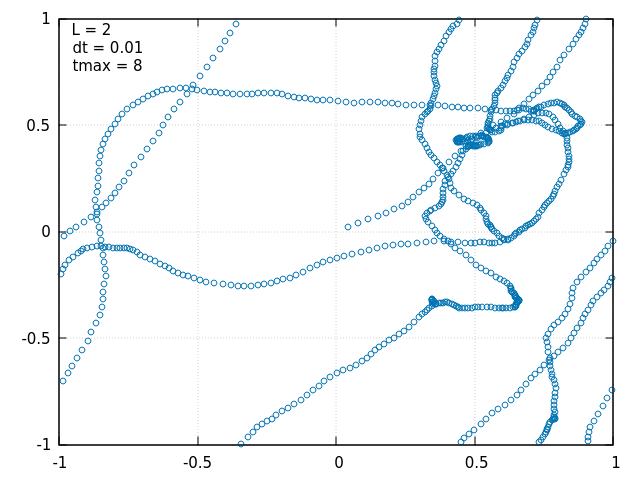
\includegraphics[width=8cm, height=6cm]{bc1.png}
      \caption{small domain size}
    \end{minipage}%
    \begin{minipage}{.5\textwidth}
      \centering
      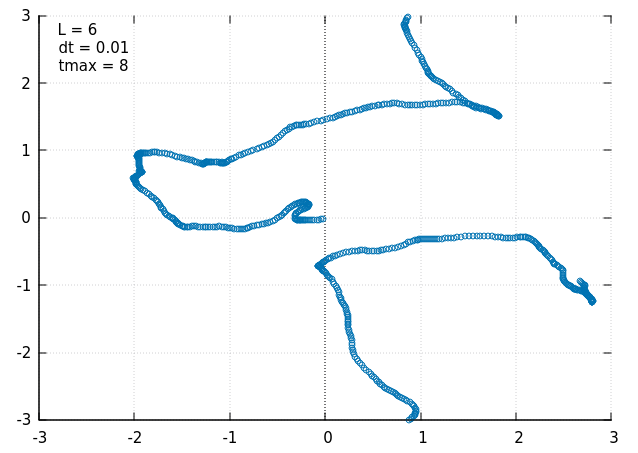
\includegraphics[width=8cm, height=6cm]{bc2.png}
      \caption{medium domain size}
    \end{minipage}
\end{figure}

\begin{figure}[!htb]
    \centering
    \begin{minipage}{.5\textwidth}
      \centering
      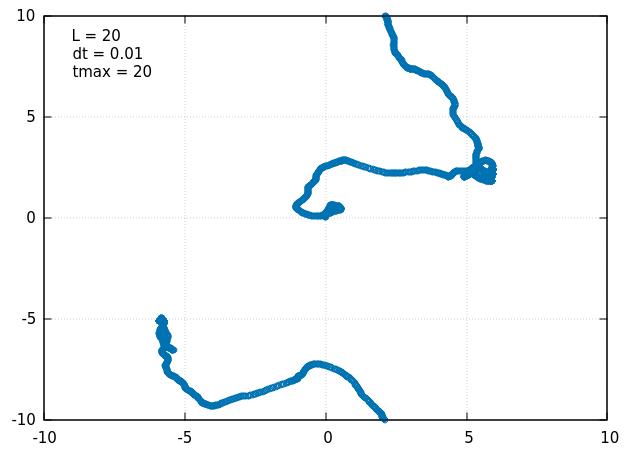
\includegraphics[width=8cm, height=6cm]{bc3.png}
      \caption{large domain size}
    \end{minipage}%
    \begin{minipage}{.5\textwidth}
      \centering
      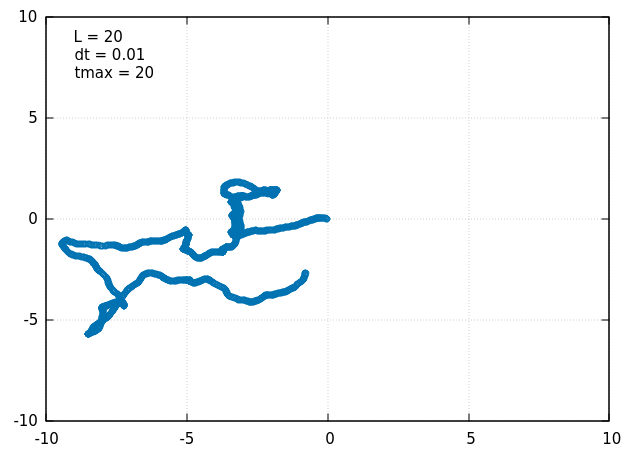
\includegraphics[width=8cm, height=6cm]{bc4.png}
      \caption{large domain size}
    \end{minipage}
\end{figure}
\newpage
\item\textbf{Pseudo-Random Forcing Implementation Test:} \\
We are using \emph{Intel MKL}\cite{mkl} library to generate random numbers with normal (Gaussian) distribution to represent noise (\(\eta\)) in the original Langevin equation. To show whether all particles are receiving different pseudo-random forcing, we draw the graph of the force received by each particle, we are using 10,000 particle for this simulation and the random force received by each particle is demonstrated for one iteration (figure 5) as well as all iterations of time (figure 6). \\
The y-axis shows the frequency of the force received by each particle. As demonstrated in the following plots, the whole distribution is Gaussian and better results are achieved when considering the whole simulation:\\

\begin{figure}[!htb]
    \centering
    \begin{minipage}{.5\textwidth}
      \centering
      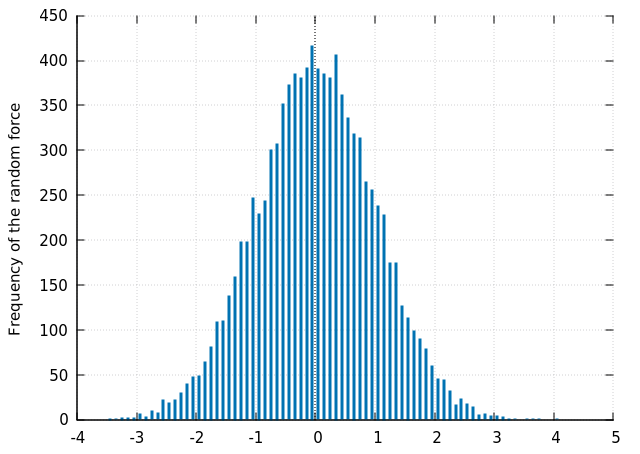
\includegraphics[width=8cm, height=6cm]{force1.png}
      \caption{\small Force distribution - single iteration}
    \end{minipage}%
    \begin{minipage}{.5\textwidth}
      \centering
      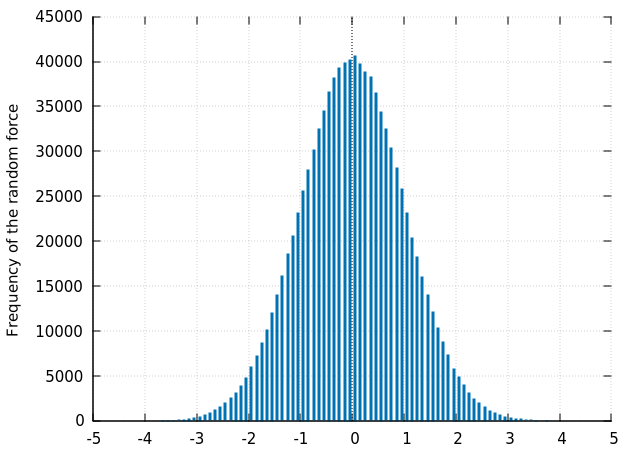
\includegraphics[width=8cm, height=6cm]{force2.png}
      \caption{\small Force distribution - total}
    \end{minipage}
\end{figure}
 
\item\textbf{Particles Distribution Test:} \\
If the size of the domain is large enough and the time-duration of our simulation is measured after a relatively long
time(\(tmax\)) then we would expect the particles distribution to be gaussian (\emph{figure 7}). If the size of domain is small, lots of particles would escape the boundaries and due to the effect of the periodic boundary condition they appear on the other side of the domain, which after a while makes the distribution of the particles more homogeneous than gaussian (\emph{figure 8}). \\
\emph{The spike at position 0 is due to the fact that in our simulations, all the particles start from point (0,0).}\\

\begin{figure}[!htb]
    \centering
    \begin{minipage}{.5\textwidth}
      \centering
      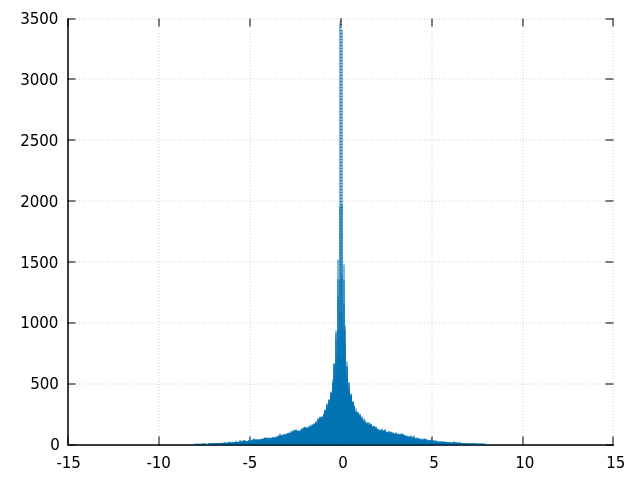
\includegraphics[width=8cm, height=6cm]{pd1.png}
      \caption{\small large domain, L = 10}
    \end{minipage}%
    \begin{minipage}{.5\textwidth}
      \centering
      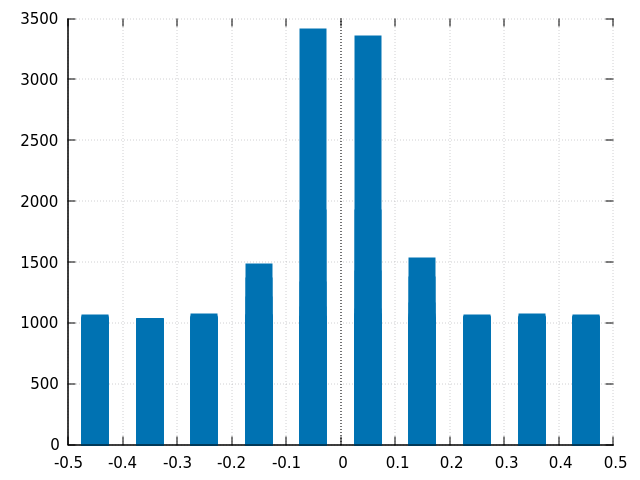
\includegraphics[width=8cm, height=6cm]{pd2.png}
      \caption{\small small domain, L = 1}
    \end{minipage}
    \caption*{Particles Distribution, n = 10,000}
\end{figure}
\newpage
To show the homogeneous distribution of the particles in a relatively small domain, we can calculate the root-mean-square displacement of the particles (\emph{figure 8}). We can see that the root-mean-square displacement of the particle gets saturated over time:

\begin{figure}[!htb]
  \centering
  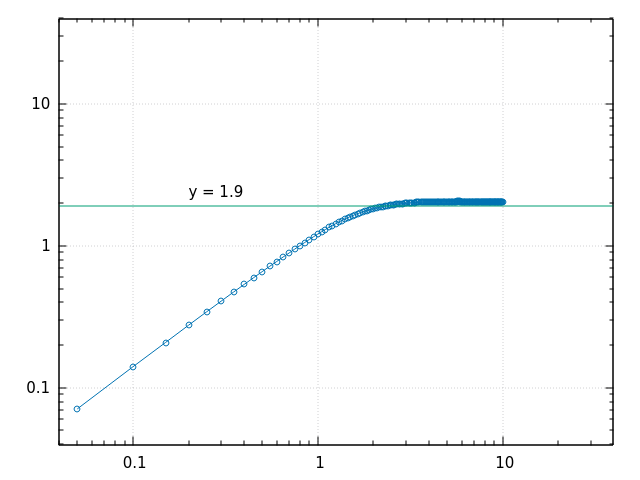
\includegraphics[width=8cm, height=5.5cm]{m1.png}
  \caption{\small root-mean-square displacement, domain size = 5}
\end{figure}
If the size of the domain is small enough or the simulation is measured after a sufficiently long time, one is able to calculate the saturation rate at time \(tmax\):

\begin{equation*}
\int_{\frac{-L}{2}}^{\frac{L}{2}} \int_{\frac{-L}{2}}^{\frac{L}{2}} \sqrt{x^2 + y^2}\ P \ dy\ dx
\end{equation*}
Where \(P\) is the probability density function (PDF) for a particle in two dimensional space and is equal to \(\frac{1}{L^2}\) when the particles displacement becomes saturated. The saturation rate in \emph{figure 9}  for \(L = 5\) is measured: \emph{( almost equal to the horizontal line drawn in figure 9)}

\begin{equation*}
\int_{-2.5}^{2.5} \int_{-2.5}^{2.5} \sqrt{x^2 + y^2}\ \frac{1}{25} \ dy\ dx = 1.91 
\end{equation*} 

\end{itemize}
\section*{Compute Autocorrelation Function:}
Velocity Autocorrelation Function (VAF) involves the velocities of the particles at two different time. To compute VAF we compare each particle's velocity with its velocity at the time origin:
\begin{equation*}
  A(\tau) = \frac{<v(0).v(\tau)>}{<v(0).v(0)>}
\end{equation*}

\begin{figure}[!htb]
    \centering
    \begin{minipage}{.5\textwidth}
      \centering
      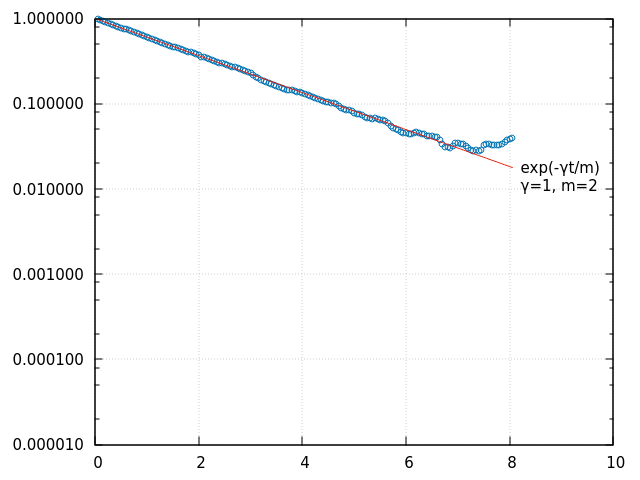
\includegraphics[width=8cm, height=6cm]{ac1.png}
      \caption{\(\frac{\gamma}{m}\) = 0.5}
    \end{minipage}%
    \begin{minipage}{.5\textwidth}
      \centering
      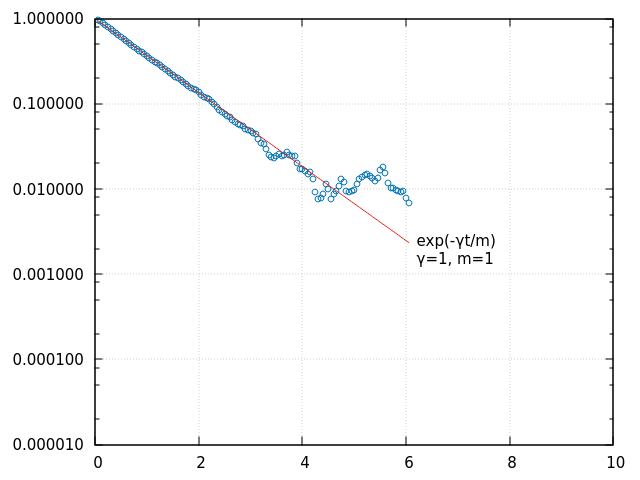
\includegraphics[width=8cm, height=6cm]{ac2.png}
      \caption{\(\frac{\gamma}{m}\) = 1}
    \end{minipage}
\end{figure}
Theory wants it that A decays as \(e^{-\gamma t/m}\). The red line in both figures above shows \(e^{-\gamma t/m}\) based on the value of \(\gamma\) and \(m\). Meaning that, as time grows we expect to experience less correlation between the velocity of a particle at the time origin and the its velocity at the measured time. Comparing \emph{figure 10} with \emph{figure 11} one can conclude that smaller values for \(\gamma/m\) means higher velocity correlation over time; that means larger values for \(m\) (more inertia) and smaller values for \(\gamma\) (less drag force) result in more correlation between the velocity of particles over time. \\
We know that the mean-square displacement of the particle gets saturated after a sufficiently long time at which the auto-correlation function of the particles decays to zero. At this point, the VAF values no longer match the \(e^{-\gamma t/m}\) graph, as shown in both graphs above. \\\\
We can demonstrate ballistic-diffusive-saturated regimes by graphing the root-mean-square displacement of the particles over a long time, showing transition from ballistic (\emph{slope = 1}) to diffusive (\emph{slope = 0.5}) scaling at a time scale \(\gamma/m\):

\begin{figure}[!htb]
    \centering
    \begin{minipage}{.5\textwidth}
      \centering
      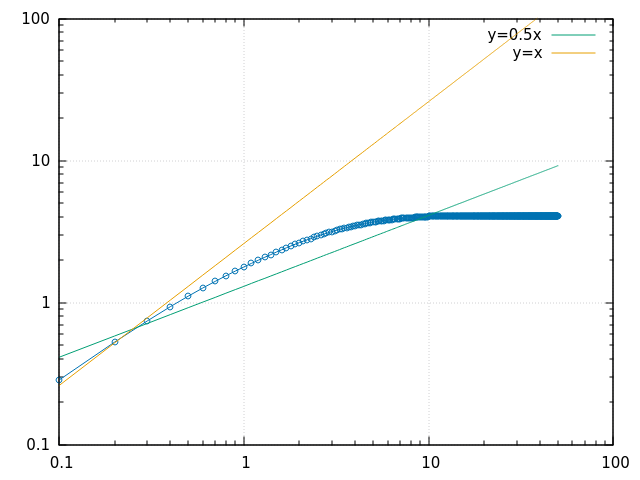
\includegraphics[width=8cm, height=6cm]{ac3.png}
      \caption{\(\frac{\gamma}{m}\) = 0.5}
    \end{minipage}%
    \begin{minipage}{.5\textwidth}
      \centering
      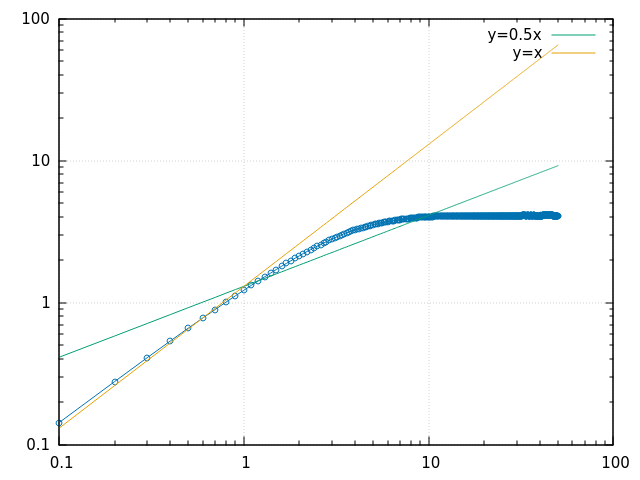
\includegraphics[width=8cm, height=6cm]{ac4.png}
      \caption{\(\frac{\gamma}{m}\) = 1}
    \end{minipage}
\end{figure}

With \(\frac{\gamma}{m} = 0.5\) (\emph{figure 12}) the transition from ballistic to diffusive happens at \(t = 0.5\), while with \(\frac{\gamma}{m} = 1\) (\emph{figure 13}) it happens at \(t = 1\).

\newpage

\begin{thebibliography}{9}

\bibitem{vectorization}
A Guide to Vectorization with Intel® C++ Compilers,
\\\texttt{https://software.intel.com/sites/default/files/m/4/8/8/2/a/
31848-CompilerAutovectorizationGuide.pdf}

\bibitem{verlet}
The Velocity Verlet algorithm,
\\\texttt{https://en.wikipedia.org/wiki/Verlet\_integration\#Velocity\_Verlet}

\bibitem{mkl}
MKL Random Number Generators,
\\\texttt{https://software.intel.com/en-us/node/521842}

\end{thebibliography}

\end{document}
